\section{Diagrama Entidad Relaci'on}

A partir de los requerimientos recabados, elaboramos un diagrama de entidad-relaci'on, que presentamos a continuaci'on.

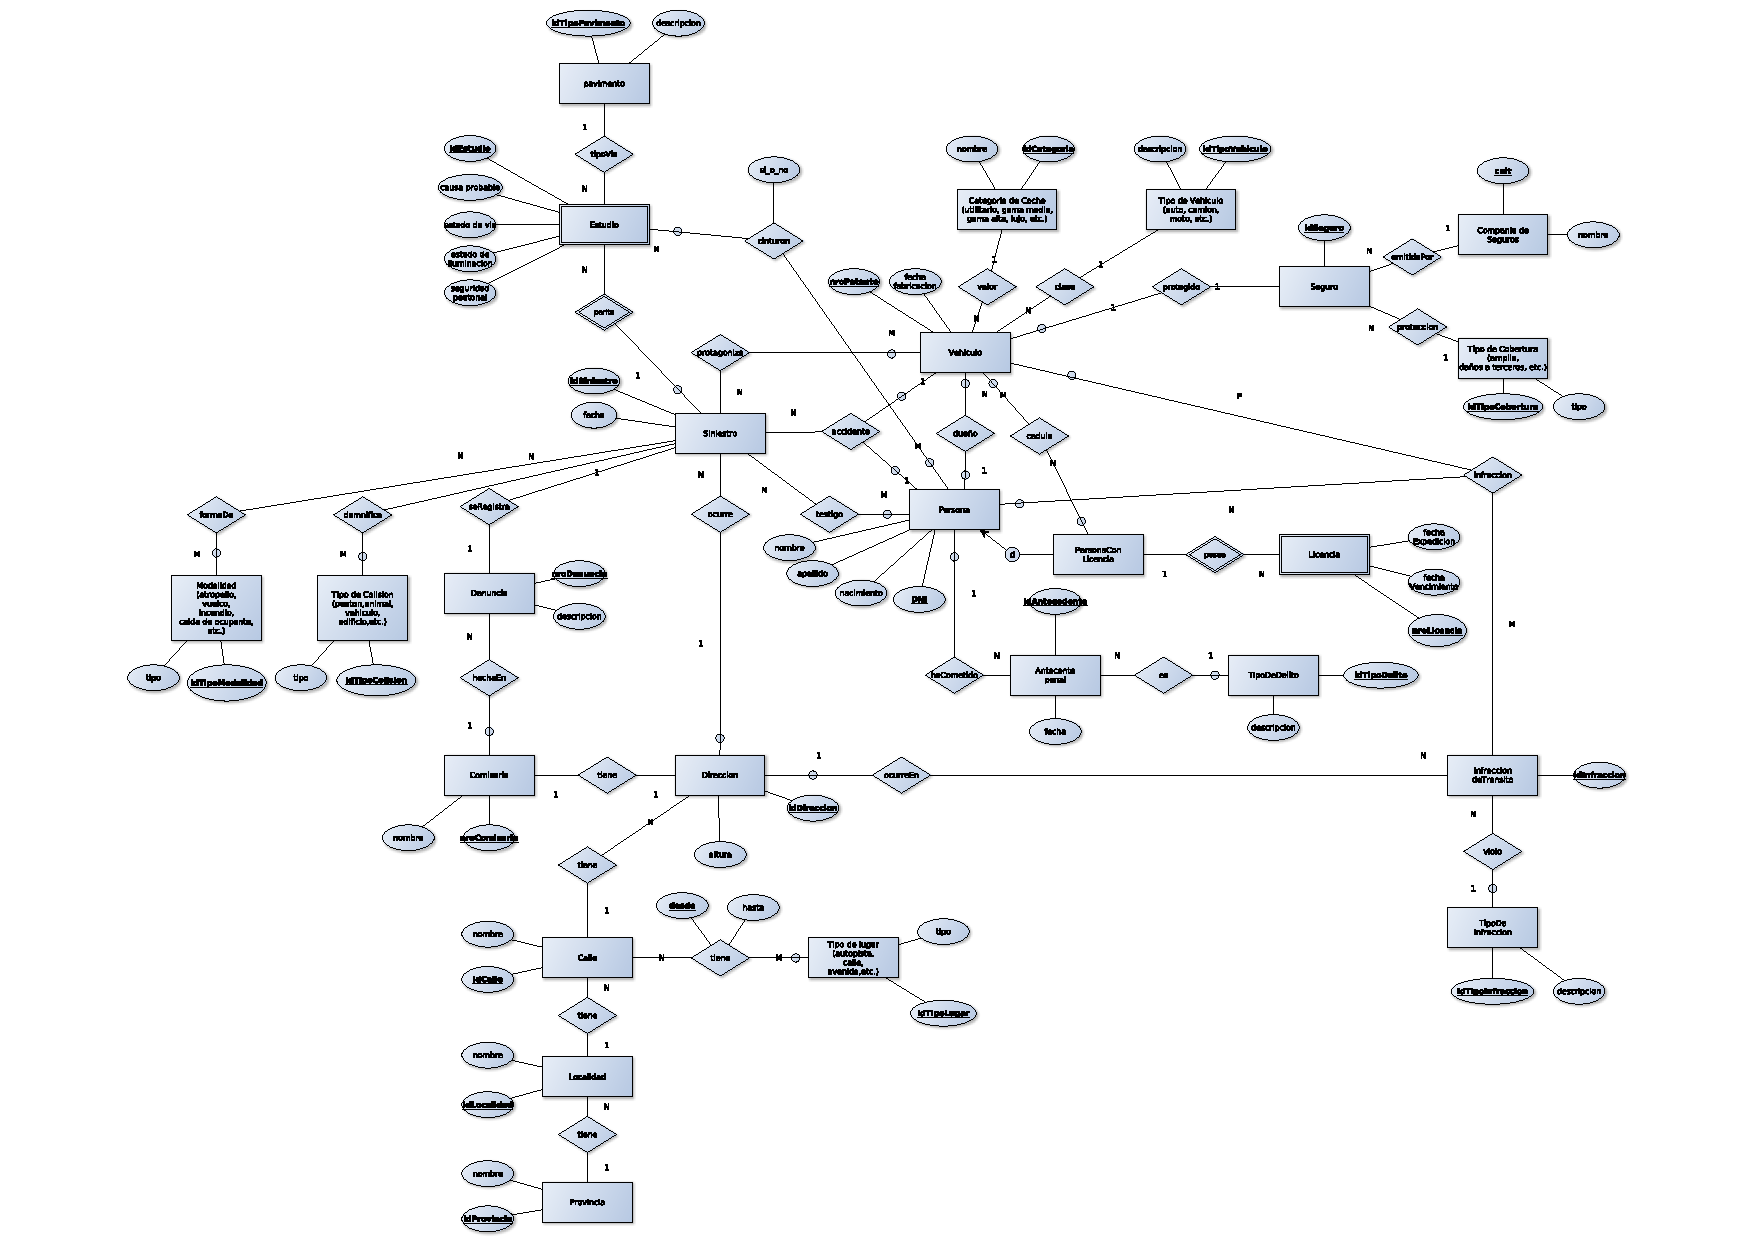
\includepdf[pages=-,angle=90]{imagenes/DER.pdf}

\subsection{Restricciones en lenguaje natural}

Las restricciones que el DER no puede capturar son las siguientes:

\begin{enumerate}
\item Las personas relacionadas con un estudio, deben estar involucradas en el siniestro correspondiente a ese estudio.

\item Si un veh'iculo sin conductor forma parte de un siniestro (es decir, est'a relacionado con un siniestro v'ia la relaci'on binaria \textit{protagoniza}), entones no era conducido por nadie en ese siniestro (es decir, no aparece en la relaci'on ternaria \textit{accidente} con ese siniestro).

\item Las personas que aparecen relacionadas con el estudio en la relacion \textit{cinturon}, deben ser personas que participaron del siniestro correspondiente al estudio, conduciendo uno de los vehiculos de ese siniestro.

\item Cada persona aparece a lo sumo una vez por siniestro. En otras palabras, un siniestro no puede estar relacionado dos veces con la misma persona v'ia la ternaria \textit{accidente}.

\item Cada vehiculo aparece a lo sumo una vez por siniestro. En otras palabras, un siniestro no puede estar relacionado dos veces con el mismo veh'iculo v'ia la ternaria \textit{accidente}.

\item No hay solapamiento entre los rangos de alturas de las calles. Por ejemplo, no puede ser que Monroe del 0 al 3000 sea calle y del 2500 al 4000 sea avenida.

\end{enumerate}
